\begin{figure}[h]
	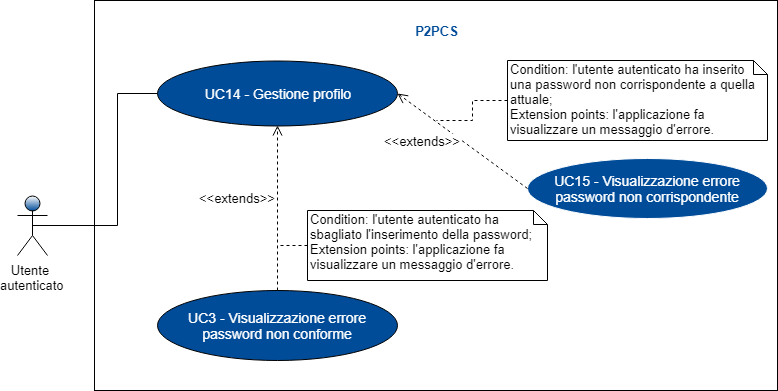
\includegraphics[width=15cm]{res/images/Schemagenerale5.png}
	\centering
	\caption{Diagramma del caso d'uso UC14 con relative estensioni (UC2, UC3, UC15)}
\end{figure}
\subsubsection{UC14 - Gestione profilo}
\begin{itemize}
	\item \textbf{Attori Primari}: utente autenticato;
	\item \textbf{Descrizione}: agli utenti autenticati è resa disponibile una maschera che presenta il proprio profilo, dalla quale l'utente può scegliere di modificarlo o eliminarlo;
	\item \textbf{Scenario principale}: l'utente visualizza il profilo e ha la possibilità di: 
	\begin{itemize}
		\item inserire la patente [UC14.1];
		\item modifica dati account [UC14.2];
		\item eliminazione account [UC14.3].
	\end{itemize}
	\item \textbf{Precondizione}: l'utente è in possesso di un account all'interno del sistema. Deve quindi essersi registrato e non aver eliminato l'account;
	\item \textbf{Postcondizione}: l'utente ha effettuato l'operazione di modifica dati oppure l'eliminazione dell'account e il processo è stato confermato dal sistema.
	\item \textbf{Estensioni}:
	\begin{itemize}
		\item visualizzazione errore email non valida [UC2];
		\item visualizzazione errore password non conforme [UC3];
		\item visualizzazione errore password non corrispondente [UC15].
	\end{itemize}
\end{itemize}
\begin{figure}[h]
	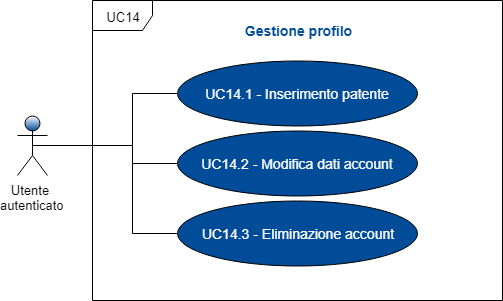
\includegraphics[width=10cm]{res/images/UC14Profilo.png}
	\centering
	\caption{UC14 - Gestione Profilo}
\end{figure}
\subsubsection{UC14.1 - Inserimento patente}
\begin{itemize}
	\item \textbf{Attori Primari}: utente autenticato;
	\item \textbf{Descrizione}: l'utente può aggiungere la propria patente al profilo;
	\item \textbf{Scenario principale}: l'utente aggiunge la patente compilando gli appositi campi obbligatori, ovvero:
	\begin{itemize}
		\item inserimento numero patente [UC14.1.1];
		\item inserimento data di rilascio e di scadenza [UC14.1.2];
		\item inserimento immagini fronte e retro della patente [UC14.1.3];
	\end{itemize}
	e successivamente salverà la patente confermando i campi appena inseriti;	 
	\item \textbf{Precondizione}: l'utente ha inserito correttamente tutti i campi necessari;
	\item \textbf{Postcondizione}: la patente viene aggiunta e visualizzata nella pagina \textit{Gestione Profilo}.
\end{itemize}
\begin{figure}[h]
	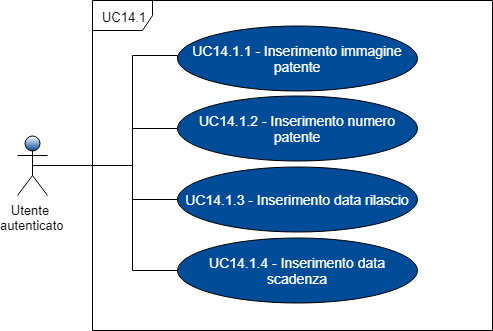
\includegraphics[width=10cm]{res/images/UC14-Patente.png}
	\centering
	\caption{UC14.1 - Inserimento patente}
\end{figure}
\newpage
\subsubsection{UC14.1.1 - Inserimento numero patente}
\begin{itemize}
	\item \textbf{Attori Primari}: utente autenticato;
	\item \textbf{Descrizione}: al fine di portare a termine il processo di inserimento della patente, l'utente deve inserire il numero della patente, campo ritenuto obbligatorio; 
	\item \textbf{Scenario principale}: l'utente compila il campo relativo al numero della patente;	
	\item \textbf{Precondizione}: l'applicazione ha reso disponibile il campo per l'inserimento del numero della patente;
	\item \textbf{Postcondizione}: l'utente ha compilato il campo con il numero della patente.
\end{itemize}
\subsubsection{UC14.1.2 - Inserimento data di rilascio e di scadenza}
\begin{itemize}
	\item \textbf{Attori Primari}: utente autenticato;
	\item \textbf{Descrizione}: al fine di portare a termine il processo di inserimento della patente, l'utente deve inserire la data di rilascio e la data di scadenza, campi ritenuti obbligatori; 
	\item \textbf{Scenario principale}: l'utente compila i campi relativi alla data di rilascio e alla data di scadenza della patente;	
	\item \textbf{Precondizione}: l'applicazione ha reso disponibile i campi per l'inserimento della data di rilascio e di scadenza della patente;
	\item \textbf{Postcondizione}: l'utente ha compilato i campi con la data di rilascio e di scadenza della patente.
\end{itemize}
\subsubsection{UC14.1.3 - Inserimento immagine fronte e retro della patente}
\begin{itemize}
	\item \textbf{Attori Primari}: utente autenticato;
	\item \textbf{Descrizione}: al fine di portare a termine il processo di inserimento della patente, l'utente deve inserire l'immagine fronte e retro della propria patente, campo ritenuto obbligatorio; 
	\item \textbf{Scenario principale}: l'utente preme il pulsante relativo all'inserimento dell'immagine della patente;	
	\item \textbf{Precondizione}: l'applicazione ha reso disponibile il bottone per l'inserimento dell'immagine della patente;
	\item \textbf{Postcondizione}: l'utente ha inserito correttamente l'immagine della patente.
\end{itemize}
\subsubsection{UC14.2 - Modifica dati account}
\begin{itemize}
	\item \textbf{Attori Primari}: utente autenticato;
	\item \textbf{Descrizione}: l'utente ha la possibilità di modificare i propri dati;
	\item \textbf{Scenario principale}: l'utente può modificare:
	\begin{itemize}
		\item nome [UC14.2.1];
		\item cognome [UC14.2.2];
		\item numero telefonico [UC14.2.3];
		\item email [UC14.2.4];
		\item data di nascita [UC14.2.5];
		\item residenza [UC14.2.6];
		\item password [UC14.2.7].
	\end{itemize}
	e confermare la modifica dei dati;
	\item \textbf{Scenari alternativi}: l'utente interrompe la modifica dei dati senza confermare il salvataggio di essi. Il sistema non salverà le modifiche parziali apportate dall'utente ma lo riporterà alla schermata di visualizzazione dell'account;	 
	\item \textbf{Precondizione}: l'utente è in possesso di un account all'interno del sistema. Deve quindi essersi registrato e non aver eliminato l'account;
	\item \textbf{Postcondizione}: il sistema ha memorizzato le modifiche apportate ai dati da parte dell’utente.
\end{itemize}
\begin{figure}[h]
	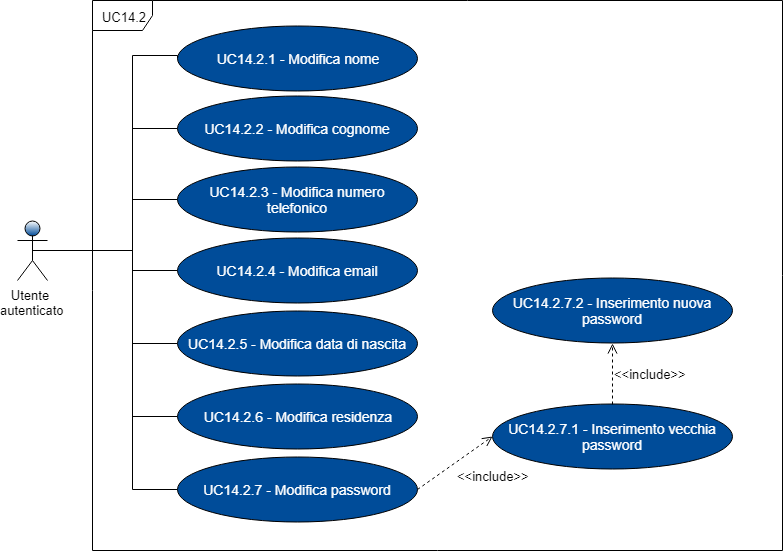
\includegraphics[width=14cm]{res/images/UC14-1Modifica.png}
	\centering
	\caption{UC14.2 - Modifica dati account}
\end{figure}
\newpage 
\subsubsection{UC14.2.1 - Modifica nome}
\begin{itemize}
	\item \textbf{Attori Primari}: utente autenticato;
	\item \textbf{Descrizione}: l'utente ha la possibilità di modificare il nome inserito in precedenza;
	\item \textbf{Precondizione}: il sistema fornisce una schermata nella quale è possibile inserire il nuovo nome;
	\item \textbf{Postcondizione}: l'utente ha inserito il nuovo nome.
\end{itemize}

\subsubsection{UC14.2.2 - Modifica cognome}
\begin{itemize}
	\item \textbf{Attori Primari}: utente autenticato;
	\item \textbf{Descrizione}: l'utente ha la possibilità di modificare il cognome inserito in precedenza;
	\item \textbf{Precondizione}: il sistema fornisce una schermata nella quale è possibile inserire il nuovo cognome;
	\item \textbf{Postcondizione}: l'utente ha inserito il nuovo cognome.
\end{itemize}

\subsubsection{UC14.2.3 - Modifica numero telefonico}
\begin{itemize}
	\item \textbf{Attori Primari}: utente autenticato;
	\item \textbf{Descrizione}: l'utente ha la possibilità di modificare il numero telefonico inserito in precedenza;
	\item \textbf{Precondizione}: il sistema fornisce una schermata nella quale è possibile inserire il nuovo numero telefonico;
	\item \textbf{Postcondizione}: l'utente ha inserito il nuovo numero telefonico.
\end{itemize}

\subsubsection{UC14.2.4 - Modifica email}
\begin{itemize}
	\item \textbf{Attori Primari}: utente autenticato;
	\item \textbf{Descrizione}: l'utente ha la possibilità di modificare l'email inserita in precedenza;
	\item \textbf{Precondizione}: il sistema fornisce una schermata nella quale è possibile inserire la nuova email;
	\item \textbf{Postcondizione}: l'utente ha inserito la nuova email.
\end{itemize}

\subsubsection{UC14.2.5 - Modifica data di nascita}
\begin{itemize}
	\item \textbf{Attori Primari}: utente autenticato;
	\item \textbf{Descrizione}: l'utente ha la possibilità di modificare la data di nascita inserita in precedenza;
	\item \textbf{Precondizione}: il sistema fornisce una schermata nella quale è possibile inserire la nuova data di nascita;
	\item \textbf{Postcondizione}: l'utente ha inserito la nuova data di nascita.
\end{itemize}

\subsubsection{UC14.2.6 - Modifica residenza}
\begin{itemize}
	\item \textbf{Attori Primari}: utente autenticato;
	\item \textbf{Descrizione}: l'utente ha la possibilità di modificare la residenza inserita in precedenza;
	\item \textbf{Precondizione}: il sistema fornisce una schermata nella quale è possibile inserire la nuova residenza;
	\item \textbf{Postcondizione}: l'utente ha inserito la nuova residenza.
\end{itemize}

\subsubsection{UC14.2.7 - Modifica password}
\begin{itemize}
	\item \textbf{Attori Primari}: utente autenticato;
	\item \textbf{Descrizione}: l'utente ha la possibilità di modificare la password inserita in precedenza inserendo prima la vecchia password e poi quella nuova;
	\item \textbf{Scenario principale}: il sistema fornisce per prima cosa all'utente la possibilità di:
		\begin{itemize}
			\item inserimento vecchia password [UC14.2.7.1].
		\end{itemize}
	e poi di:
		\begin{itemize}
			\item inserimento nuova password [UC14.2.7.2].
		\end{itemize}
	\item \textbf{Precondizione}: il sistema fornisce una schermata nella quale è possibile inserire la nuova password;
	\item \textbf{Postcondizione}: l'utente ha inserito la nuova password.
\end{itemize}

\subsubsection{UC14.2.7.1 - Inserimento vecchia password}
\begin{itemize}
	\item \textbf{Attori Primari}: utente autenticato;
	\item \textbf{Descrizione}: l'utente deve inserire la password attuale per poterla aggiornare;
	\item \textbf{Precondizione}: il sistema fornisce una schermata nella quale è possibile inserire la vecchia password;
	\item \textbf{Postcondizione}: l'utente ha inserito la vecchia password.
\end{itemize}

\subsubsection{UC14.2.7.2 - Inserimento nuova password}
\begin{itemize}
	\item \textbf{Attori Primari}: utente autenticato;
	\item \textbf{Descrizione}: l'utente deve inserire la nuova password per effettuare l'aggiornamento;
	\item \textbf{Precondizione}: il sistema fornisce una schermata nella quale è possibile inserire la nuova password;
	\item \textbf{Postcondizione}: l'utente ha inserito la nuova password.
\end{itemize}

%\subsubsection{UC14.2.8 - Conferma modifica dati}
%\begin{itemize}
%	\item \textbf{Attori Primari}: utente autenticato;
%	\item \textbf{Descrizione}: l'utente deve 
%	confermare la modifica apportata;
%	\item \textbf{Precondizione}: l'utente ha inserito tutti i dati richiesti e desiderati. Si trova dunque davanti ad una schermata con la possibilità di confermare la modifica effettuata;
%	\item \textbf{Postcondizione}: l'utente ha confermato di voler rendere effettivo il cambiamento del proprio account.
%\end{itemize}

\subsubsection{UC14.3 - Eliminazione account}
\begin{itemize}
	\item \textbf{Attori Primari}: utente autenticato;
	\item \textbf{Descrizione}: all'utente viene fornita la possibilità di eliminare il proprio account e di conseguenza i propri dati all'interno del sistema;
	\item \textbf{Precondizione}: l'utente è in possesso di un account all'interno del sistema. Deve quindi aver effettuato la registrazione e non avere mai effettuato la procedura di eliminazione account;
	\item \textbf{Postcondizione}: l'utente ha cancellato il proprio account e viene riportato alla schermata iniziale dell'applicazione [UC1]. Il sistema non terrà traccia del profilo eliminato.
\end{itemize}

\subsubsection{UC15 - Visualizzazione errore password non corrispondente}
\begin{itemize}
	\item \textbf{Attori Primari}: utente autenticato;
	\item \textbf{Descrizione}: l'utente visualizza un messaggio d'errore in quanto la password digitata in [UC14.2.7.1] non corrisponde alla vecchia password;
	\item \textbf{Scenario principale}: l'utente autenticato cerca di cambiare la password del proprio account;
	\item \textbf{Precondizione}: l'utente autenticato ha inserito una password non corrispondente a quella attuale;
	\item \textbf{Postcondizione}: l'applicazione fa visualizzare un messaggio d'errore.
\end{itemize}



